\documentclass[../mit-general-chemistry.tex]{subfiles}
\begin{document}



\chapter{Chemical equilibrium}





Chemical reactions reach a state of chemical equilibrium in which the
rate of forward and reverse reactions are equal and there is no net
change in composition.


\section{Nature of chemical equilibrium}

Consider the Haber process

\ceeq{N2(g) + 3H2(g) <=> 2NH3(g)\label{rxn:amonia}}


Say we start with a mixture of nitrogen gas and hydrogen gas. In a
diagram of the concentrations of reactants and product over time we
would see the concentrations of the reactants decrease as the reaction
progres and then level off.

Initially, we have pure reactants and the reaction is spontaneous in
the forward direction. We can tell that $\gibbs < 0$ as this is a
forward reaction.

\begin{center}
  \begin{tikzpicture}
    \begin{axis}[
        width=6cm,
        height=6cm,
        xlabel = time,
        ylabel = concentration,
        axis lines = left,
        xmin=0,
        xmax=10,
        ymin=0,
        ymax=10,
        xtick = {},
        ytick = {},
        xticklabels = \empty,
        yticklabels = \empty,
        clip = false,
      ]
      \draw[blue] (0,9) to[curve through={(1,8) .. (2, 7.5) .. (3, 7)}] (10, 5.8);
      \draw[blue] (0,8) to[curve through={(1,7) .. (2, 6.5) .. (3, 6)}] (10, 5);
      \draw[red!50!black] (0,0) to[curve through={(1,1) .. (2, 1.5)}] (10, 2.8);
    \end{axis}
  \end{tikzpicture}
\end{center}


If you would have pure products, then the reaction would be
spontaneous in the reverse direction and $\gibbs > 0$.


We interpreted Gibb's free energy in terms of stable or unstable
products relative to reactants. When $\gibbs < 0$, the product is more
stable than the reactants and vice versa.


\begin{center}
  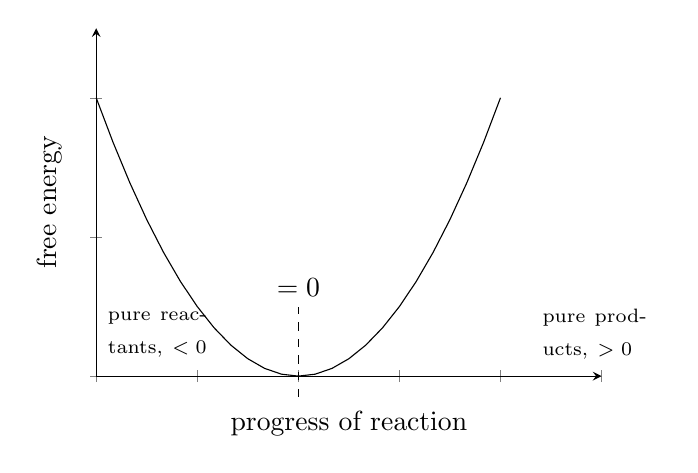
\begin{tikzpicture}
    \begin{axis}[
        width=8cm,
        height=6cm,
        xlabel = progress of reaction,
        ylabel = free energy,
        axis lines = left,
        xmin=0,
        xmax=5,
        ymin=0,
        ymax=5,
        xtick = {},
        ytick = {},
        xticklabels = \empty,
        yticklabels = \empty,
        clip = false,
      ]
      \addplot[domain=0:4]{(x - 2)^2};
      \draw[dashed] (2, -0.3) -- (2, 1)
      node[at end,above]{$\gibbs = 0$};
      \node[text width=1.5cm] at (axis cs:.7, .6) {\scriptsize pure reactants, $\gibbs < 0$};
      \node[text width=1.5cm] at (axis cs:5, .6) {\scriptsize pure products, $\gibbs > 0$};
    \end{axis}
  \end{tikzpicture}
\end{center}


If we have pure reactants and $\gibbs < 0$. Reaction~\ref{rxn:amonia} will
progress, the reactants will spontaneously form products and the free
energy will decrease.

On the other hand, if we have a state of pure reactants, \gibbs will
be greater than zero. Now, products will spontaneously dissolve into
the reactants.

This will happen until the system reaches equilibrium. So \gibbs is
closely related to the notion of chemical equilibrium.

The reaction free energy ($\gibbs_r$) chamges as the proportions of
reactants and products change.


This is reflected in the equation
\begin{equation}\label{eq:free-energy}
  \gibbs = \gibbs^0 + RT \ln Q
\end{equation}

Where

\begin{center}
  \begin{tabularx}{.67\textwidth}{lX}
    \gibbs & Reaction free energy at any definite fixed composition of
    the reaction mixture. \\
    $\gibbs^0$ & The difference in molar free energy of the products
    on one hand, and reactants on the other, in their standard
    states. \\
    $Q$ & Reaction quotient. \\
    $R$ & Universal gas constant. \\
    $T$ & Temperature (K). \\
  \end{tabularx}
\end{center}





The reaction quotient, $Q$, os calculated in different way depending
on whether it occurs in a gaseous state or in solution.

For some reaction

\ceeqstar{aA + bB <=> cC + dD}

When reactants and prodicts are in a gasous state the reaction
quotient is defined as
\begin{equation}
  Q =
  \left[
    \frac{
      \left( \frac{P_C}{P_{\text{ref}}} \right)^c
      \left( \frac{P_D}{P_{\text{ref}}} \right)^d
    }{
      \left( \frac{P_A}{P_{\text{ref}}} \right)^a
      \left( \frac{P_B}{P_{\text{ref}}} \right)^b
    }
    \right]
\end{equation}
where $P_{\text{ref}}$ is a reference partial pressure. Under standard
conditions $P_{\text{ref}} = \SI{1}{\bar}$. Under those conditions
\begin{equation}
  Q =
  \frac{
    (P_C)^c
    (P_D)^d
  }{
    (P_A)^a
    (P_B)^b
  }
\end{equation}


In solution the reaction quotient is defined by
\begin{equation}
  Q = \frac{
    \left( \frac{[C]}{C_{\text{ref}}} \right)^c
    \left( \frac{[D]}{C_{\text{ref}}} \right)^d
  }{
    \left( \frac{[A]}{C_{\text{ref}}} \right)^a
    \left( \frac{[B]}{C_{\text{ref}}} \right)^b
  }
\end{equation}
for the concentrations of the reactants and products.

For a refernce concentration, $C_{\text{ref}}$, of \SI{1}{\mol} the
equations is simplified
\begin{equation}
  Q = \frac{ [C]^c [D]^d }{ [A]^a [B]^b }
\end{equation}











\section{Meaning of $K$}



At equilibrium $\gibbs = 0$ and $Q = K$, the equilibrium constant. For
$\gibbs = 0$ we can solve Equation~\ref{eq:free-energy} for $\gibbs^0$
\begin{align*}
  \gibbs &= \gibbs^0 + RT \ln Q \\
  0 &= \gibbs^0 + RT \ln K & \text{for } \gibbs = 0 \\
  \gibbs^0 &= -RT \ln K \\
\end{align*}

$K$ is the equilibrium constant. $K = Q$ at equilibrium as in the
equations above. It has the same form as $Q$ but only uses the amounts
of reactants and products at equilibrium.






\section{Relationship between equilibrium expressions}




Now, we can rewrite Equation~\ref{eq:free-energy} one more time
\begin{equation}
  \gibbs = \gibbs^0 + RT \ln Q = -RT \ln K + RT \ln Q = RT \ln\left(\frac{Q}{K}\right)
\end{equation}

Lets think about the factor $\ln\left(\frac{Q}{K}\right)$ for a
minute. If $Q < K$ then $\gibbs < 0$ and the forward reaction will
occur. If $Q > K$ then $\gibbs > 0$ and the reverse reaction will
occur.


\begin{example}
  If $K = \num{1.9d-4}$ at \SI{400}{\kelvin} and
  \begin{center}
    \begin{tabular}{ll}
      $P_{\ce{NH3}}$ & \SI{1.1}{\bar} \\
      $P_{\ce{N2}}$ & \SI{5.5}{\bar} \\
      $P_{\ce{H2}}$ & \SI{2.2}{\bar} \\
    \end{tabular}
  \end{center}
  also at \SI{400}{\kelvin}.

  Now consider
  \ceeqstar{N2(g) + 3H2(g) <=> 2NH3(g)\tag{a}}

  Which direction will the reaction go?

  Lets calculate
  \begin{align*}
    Q &= \frac{(P_{\ce{NH3}})^2}{(P_{\ce{N2}})(P_{\ce{H2}})^3} =
    \frac{(1.1)^2}{(5.5)(2.2)^3} =
    \num{2.067d-2} > K
  \end{align*}

  Now, since $Q > K$ under these conditions
  \begin{equation*}
    \ln\left(\frac{Q}{K}\right) > 0
  \end{equation*}
  and the reaction will go in the
  reverse direction, forming nitrogen gas and hydrogen gas from ammonia
  gas. Ammonia will dissociate until equilibrium is reached.
\end{example}


What does $K$ tell us? It tells us the mixture of reactants and
products at equilibrium, wether we can expect high or low
concentration of products at equilibrium.

\begin{equation*}
  K = \left[ \frac{\text{products}}{\text{reactants}} \right]_{\text{equilibrium}}
\end{equation*}

When $K > 1$ we will find a high concentration of products at
equilibrium and conversively when $K < 1$ we will find a low (-er)
concentration of products at equilibrium. This comes, naturally, from





For $K > 1$
\ceeqstar{2NO2 <=> N2O4}

This reaction has $\gibbs^0 = \SI{-4.76}{\kilo\joule\per\mol}$ and $K
= 6.84$ at \SI{298}{\kelvin}.

Initially, we start with a pressure at \SI{1}{\bar} of \ce{NO2}
(reactants) and no \ce{N2O4} (product).


\begin{center}
  \begin{tikzpicture}
    \begin{axis}[
        width=8cm,
        height=6cm,
        xlabel = progress of reaction (time),
        ylabel = partial pressure (\si{\bar}),
        axis lines = left,
        xmin=0,
        %xmax=2,
        ymin=0,
        ymax=4,
        xtick = {},
        ytick = {2.5},
        xticklabels = \empty,
        yticklabels = 1,
        clip = false,
      ]
      \addplot[domain=0.001:10]{1/(x + .5) + .5}
      node[pos=.9, above]{\ce{NO2} (reactant)};
      \addplot[domain=0.001:10]{2 - (1/(x + .5))}
      node[pos=.9, above]{\ce{N2O4} (product)};
    \end{axis}
  \end{tikzpicture}
\end{center}


Early on, we have no products in the reaction mix. This means that $Q
< K$ which in turn yields $\gibbs < 0$. This makes the reaction
spontaneous in the forward direction, which means the reactants start
to form products.


So, what will be the concentrations at equilibrium? We can go ahead
and calculate this.
\begin{center}
  \begin{tabular}{llll}
    & \ce{2NO2} & \ce{<=>} & \ce{N2O4} \\
    initial pressure & 1 & & 0 \\
    change & $-2x$ & & $+x$ \\
    equilibrium & $1 - 2x$ && $x$ \\
  \end{tabular}
\end{center}

Now, we know $K = 6.84$, so let us plug this in
\begin{equation*}
  K = 6.84 = \frac{P_{\ce{N2O4}}}{(P_{\ce{NO2}})^2}
  = \frac{x}{(1 - 2x)^2}
\end{equation*}

Solving this for $x$ we get $x = \SI{0.381}{\bar}$. From our
calculations we can plug this in and find the concentrations at
equilibrium.
\begin{align*}
  P_{\ce{NO2}} &= 1 - 2x = 1 - 2(0.381) = \SI{0.238}{\bar} \\
  P_{\ce{N2O4}} &= x = \SI{0.381}{\bar} \\
\end{align*}


We see that, at equilibrium, we have more product than reactants which
is consistent with $K > 1$.


It is easyly understood from  Equation~\ref{eq:free-energy} that
\begin{equation}
  \gibbs^0 = -RT \ln K \quad\Leftrightarrow\quad K = e^{ - \frac{\gibbs^0}{RT}}
\end{equation}
and that this suggests that $K$ is large if $\gibbs^0$ is large and
negative. If $K$ is a large, positive number, then there is going to
be a lot of products and not so much reactants and vice versa.




If the overall reaction can be written as a {\em sum} of two or more
chemical equations, the equilibrium constant for the overall reaction
is the {\em product} of the equilibrium constants for the component
reactions.


\begin{align*}
  &\ce{2P(g) + 3Cl2(g) <=> 2PCl3(g)} &K_1 \tag{a}\\
  &\ce{PCl3(g) + Cl2(g) <=> PCl5(g)} &K_2 \tag{b}\\
  &\ce{2P(g) + 5Cl2(g) <=> 2PCl5(g)} &K_3 \tag{c}\\
\end{align*}


We see that we can write an formula of the first two equations to
obtain the third as $a + b + b = a + 2b = c$. If $K_1$ and $K_2$ are
known, we can calculate $K_3 = K_1 \cdot K_2^2$. Since we add $b$
twice, we need to take $K_2$ to the second power when we're
multiplying the equilibrium constants.




\section{External effects on the relationship of $Q$ and $K$}


\begin{definition}[Le Châtelier's principle]
  A system in equilibrium that is subjected to stress will react in a
  way that tends to minimize the effect of that stress.
\end{definition}

{\em Stress of a system} is a change of the circumstances surrounding
the system that disturbs the equilibrium of that system.

La Châtelier's principle predict a way to, qualitatively, predict the
direction of change of a system under an external influence or
perturbation.






\subsection{Adding and removing reactants and products of the system}


One way to add stress to a system is to add to or remove from it. This
disturbs the equilibrium.

Consider, again,
\ceeqstar{N2(g) + 3H2(g) <=> 2NH3(g)}

If we add some more hydrogen gas to this system after it has reached
equilibrium, two things will happen. The first thing is that the two
reactants will for more product. Since this requires both reactants,
thís will consume both hydrogen gas and nitrogen gas. We will thus see
a decrease in nitrogen gas as ammonia is formed. All this occurs in a
way that equilibrium is reached again, $Q = K$ again.

In the same way, if we would add some of the product to the
system. More ammonia would dissociate into reactants until the
proportions of the reactants and the product ($Q$) again mounts up to
the equilibrium constant ($K$) so that $Q = K$.

If you are in equilibrium, adding more hydrogen gas, the system will
tend to minimize the increase. Reaction shift to right ``toward
product''.

If the system is at equilibrium $Q = K$. When we add to one of the
reactants $Q$ is decreased momentarily, $Q < K$. Then \gibbs is
decreased. We remember that $\gibbs < 0$ makes a reaction spontaneous
to the right so the system start to form more product.

Conversely, if we add more ammonia to the system, $Q =
\frac{[\text{products}]}{[\text{reactants}]}$ will increase and this
makes $\gibbs > 0$. So the reaction will dissociate product into
reactants as a consequence.





\subsection{Changing the volume}


A decrease of the volume of a system increases the total pressure of
that system.

The ideal gas law jumps to mind
\begin{equation}
  PV = nRT
\end{equation}

Le Châtelier's principle predicts that the system will respond to an
increase in pressure in a way as to reduce the total pressure.


As an example, consider the reaction \ceeqstar{2P2(g) <=> P4(g)}

We could take a mixture of the gasses in a sealed container. We
assume the mix has reached equilibrium. We can then decrease the
volume, and thus increase the pressure. This would cause the
reaction to tend towards product, since there are two moles of
reactant for every mole of product and this releases pressure.


In the terms of $Q$ and $K$, suppose the volume of the container is
decreased by half (a factor of two). This will increase the partial
pressure of both gasses by a factor of two, initially. Before the
stress is applied to the system, $Q = K$. When we apply the pressure
and the partial pressures of the gasses are doubled. Let $p_r$ be the
partial pressure of the reactant at equilibrium and $p_p$ be the
partial pressure of the product at equilibrium. At equilibrium
\begin{equation*}
  Q = K = \frac{p_p}{(p_r)^2}
\end{equation*}
When we apply the stress to the system and decrease the volume of the
container $Q$ changes accordingly
\begin{equation*}
  Q = \frac{2p_p}{(2p_r)^2} = \frac{p_p}{2p_r} < \frac{p_p}{p_r} = K
\end{equation*}

So the denominator will increase more from the stress than the
nominator will. As $Q < K$ which yields $\gibbs < 0$ the reaction will
tend toward product until $Q = K$ again.

If we instead increase the volume and thus decrease the pressure
inside the container we will have the opposite effect. Let's say we
decrease the pressure inside the container by half, a factor of
two. At equilibrium
\begin{equation*}
  Q = K = \frac{p_p}{(p_r)^2}
\end{equation*}

When we decrease the total pressure of the container, we half the
partial pressures of the gasses, so
\begin{equation*}
  Q = \frac{\frac{1}{2}p_p}{(\frac{1}{2}p_r)^2}
  = \frac{p_p}{\frac{1}{2}p_r}
  = 2\frac{p_p}{p_r}
  > \frac{p_p}{p_r} = K
\end{equation*}

And similarly to last example, as $Q > K$ the reaction tends toward
reactants and dissociating product until $Q = K$ again.



We should be aware of the fact that $Q$ depends of the quotient of the
partial pressures of the reactants and the products of a reaction. If
we insert an inert gas into the container, this affects the partial
pressures equally and does not affect $Q$ and will, thus, not disturb
the equilibrium.



\begin{hfigure}
  \begin{remark}
    \textbf{Review: partial pressure}
    
    The partial pressure of a gas, possibly in a mixture of gasses, in a
    container is the pressure that gas would exert on the container if
    it was alone in the container.

    Let's say we have a volume of \ce{O2(g)} with $P_{\ce{O2}} =
    \SI{1}{\bar}$ and we have an equal volume of \ce{N2(g)} with
    $P_{\ce{N2}} = \SI{1}{\bar}$. If those two amounts of the gasses
    were put inside the same volume, the total pressure would be
    \SI{2}{\bar}. The partial pressure of each gas is \SI{1}{\bar}
    whether the other gas is present or not.

    We have the equation
    \begin{equation}
      P_A = n_A \frac{RT}{V}
    \end{equation}
    the partial pressure for the gas \ce{A}. $n_A$ being the number of
    moles of gas; $R, T$ and $V$ as expected.

    The total pressure of a gas mixture on it's container is the sum of
    the partial pressures of the gasses on that container.
    \begin{equation}
      P_{\text{tot}} = \sum_i \left(n_i\frac{RT}{V}\right)
      = \frac{RT}{V}\cdot\sum_i n_i
      = \frac{RT}{V} n_{\text{tot}}
    \end{equation}
  \end{remark}
  \caption{Review of the concept of partial pressure.}
\end{hfigure}





\subsection{Changing the temperature}


Raising the temperature of a mixture in equilibrium by adding heat
causes the reaction to shift in such a way that some of the heat is
absorbed. This is consistent with Le Châteliers principle. Here the
enthalpy change (\enthalpy) of a reaction is the predictive tool when
thinking about the direction of change when adding heat to a system.



Let's consider the effect of raising the temperature of an {\em
  exothermic} reaction ($\enthalpy < 0$), a reactions that releases
heat to the surroundings. Such a reaction tends to the reactants to
absorb the extra heat, it favors the forming of reactants.

For an exothermic reaction
\ceeqstar{{\text{reactants}} <=>[{heat produced}][{heat absorbed}] {\text{products}}}


If we add heat, the system will go in a direction that will absorb
that heat.

For an {\em endothermic} reaction ($\enthalpy > 0$) that absorbs heat
from the surroundings to proceed to the right, the effect of
adding heat is the opposite from the example above
\ceeqstar{{\text{reactants}} <=>[{heat absorbed}][{heat produced}] {\text{products}}}
so increasing the temperature of the system favors formation of
products.

We know from the definition of the notion of endothermic reactions
that an endothermic reaction is a reaction that {\em requires energy
  to occur} (going forward, to the right). Here we actually add that
heat.




\begin{example}
  Consider
  \ceeqstar{2SO2(g) + O2 <=> 2SO3(g)}

  Enthalpy for this reaction is $\enthalpy^0 =
  \SI{-197.78}{\kilo\joule\per\mol}$ \ce{O2}.

  If we add heat to this reaction when it has reached equilibrium,
  what direction will the reaction go?

  As $\enthalpy^0 < 0$ this is a exothermic reaction and adding heat
  will make it tend toward the reactants.
\end{example}




\subsection{The dependence of $K$ on temperature}


So far we have looked at the equilibrium constant at constant
temperatures. But $K$ actually depends on the temperature and changes
with it. Reaction rates also changes with temperature.

So what is the relation between the equilibrium constant and the
temperature? We have already seen the two relations
\begin{align*}
  \gibbs^0 &= -RT \ln K \\
  \gibbs^0 &= \enthalpy^0 - \dS T \\
\end{align*}
The two left hand sides is obviously equal so we conclude that the two
right hand sides are equal and
\begin{equation}\label{eq:lnk}
  \ln K = - \frac{\enthalpy^0}{RT} + \frac{\dS^0}{R}
\end{equation}

It is assumed that $\enthalpy^0$ and $\dS^0$ is relatively independent
of the temperature, as this changes within ``temperatures of interest
to us'', so we're safe to say that $K$ changes with a change in $T$.


Consider now a reaction carried out at two temperatures $T_1$ and
$T_2$. Plugging this in into Equation~\ref{eq:lnk}
\begin{align*}
  \ln K_1 &= -\frac{\enthalpy^0}{RT_1} + \frac{\dS}{R}\quad\text{and}\\
  \ln K_2 &= -\frac{\enthalpy^0}{RT_2} + \frac{\dS}{R}\\
\end{align*}

Subtracting $K_1$ from $K_2$ give us a measure ($\Delta K$) of the
impact a temperature change from $T_1$ to $T_2$ have on the
equilibrium constant
\begin{equation}\label{eq:van't hoff}\tag{Van't Hoff equation}
  \Delta K = \ln K_2 - \ln K_1 = \ln\left(\frac{K_2}{K_1}\right) = - \frac{\enthalpy^0}{R}~\left[\frac{1}{T_2} - \frac{1}{T_1}\right]
\end{equation}

In this section we will notice that the sign of $\Delta K$ tells us
whether $K_2 > K_1$ (less reactants, more product) or $K_2 < K_1$
(more reactants, less product) after the change in temperature.


Consider a case of an exothermic reaction, $\enthalpyO < 0$. That
means that the factor $- \frac{\enthalpy^0}{R} > 0$.

We begin with looking at the case where we are going to increase the
temperature, $T_2 > T_1$.

We have
\begin{equation*}
  \left[\frac{1}{T_2} - \frac{1}{T_1}\right] < 0
\end{equation*}
since $T_2 > T_1$ and thus
\begin{equation*}
  \ln\left(\frac{K_2}{K_1}\right) < 0
  \implies \frac{K_2}{K_1} < 1
  \implies K_2 < K_1
\end{equation*}
and this means that the quotient of product to reactants have
decreased so the reaction tends toward reactants.

In the same manner, if $\enthalpyO < 0$ (exothermic reaction) and $T_2
< T_1$ (decreased temperature), we get $K_2 > K_1$ which means more
products, The reaction tends toward products.

When we look at endothermic reactions, that just means another switch
of signs as $\enthalpy^0 > 0$ (reaction requires energy to occur). A
system of reactants that absorbs heat from the surroundings in an
endothermic reaction has a positive \enthalpy, because the enthalpy of
the products is higher than the enthalpy of the reactants of the
system. If we only look at the equation and the sign of the factors, a
positive \enthalpy means the first factor ($-\frac{\enthalpy^0}{RT}$)
is negative. Now the second factor (within brackets) is positive when
$T_2 < T_1$, a decrease in temperature and negative when $T_2 > T_1$,
a increase in temperature. We can conclude that for endothermic reactions
$\Delta K > 0$ (more products) if we decrease the temperature and
$\Delta K < 0$ (more reactants) if we increase the temperature. We can
conclude this simply by looking at the equation.

The table below 
\begin{htable}
  \begin{center}
    \begin{tabularx}{.8\textwidth}{XXX}
      \toprule
      Reaction is & \specialcell{$T_2 < T_1$\\ (decrease)} & \specialcell{$T_2 > T_1$\\ (increase)} \\
      \midrule
      \specialcell{Exothermic\\ $\enthalpy^0 < 0$} &
      \specialcell{$K_2 < K_1$\\ more reactants} &
      \specialcell{$K_2 > K_1$\\ more products} \\
      \\
      \specialcell{Endothermic\\ $\enthalpy^0 > 0$} &
      \specialcell{$K_2 > K_1$\\ more products} &
      \specialcell{$K_2 < K_1$\\ more reactants} \\
      \bottomrule
    \end{tabularx}
  \end{center}
  \caption{The relationship between temperature; thermodynamics and
    the effect of temperature change.}
\end{htable}





\section{Examples of chemical equilibrium}






\subsection{Maximizing the yield of a reaction}


If we were to design an industrial process we could use our new
knowledge from the last two chapters to maximize the outcome from
certain reactions.

Consider
\ceeqstar{N2(g) + 3H2(g) <=> 2NH3(g)}

This is an exothermic reaction ($\enthalpyO < 0$), which means that
low temperature favors products, but also slows reaction rate down (as
we shall see in chapter on kinetics) so we would need to compromise
and so people do. Ammonia tends to be produces at \SI{500}{\celsius}.

In the equation of the reaction, on the stoichiometric coefficients,
that there are four moles of gas of reactants and two moles of gas of
the product. The forward reaction would be favored if we increased the
pressure within the container harboring the process.

Removing ammonia during the process would also favor forming of more
ammonia.


People are also working on designing enzymatic processes to replace
the Haber-Bosch process of high temperature and high pressure.

The enzyme {\em nitrogenase} is able to split \ce{N2} molecules into
two nitrogen atoms using transition metals. This is a hot research
topic in chemistry today.




\subsection{Oxygen and hemoglobin}


The combination of oxygen with hemoglobin (Hb) which carries oxygen
through the blood can be represented by
\ceeqstar{Hb(aq) + O2(aq) <=> HbO2(aq)}
where \ce{HbO2} is oxyhemoglobin which is oxygen bound to hemoglobin.

If we travel to higher altitudes, the partial pressure of oxygen in
the atmosphere will decrease, At an altitude of \SI{3}{\kilo\meter}
the partial pressure of oxygen is \SI{0.14}{\atm} compared to
\SI{0.2}{\atm} at sea level.

At a lower partial pressure of oxygen the reaction above will tend
towards reactants, so less hemoglobin will be bound to hemoglobin in
the body.

The body will, however, react to this new situation and start
producing more hemoglobin as this will result in more product being
formed.







\end{document}
